% MADEVO -- draft paper. Build: pdflatex main && bibtex main && pdflatex main && pdflatex main
% Every number comes from ~/madevo_final_2411/ (final campaign, 2026-11-24) and from the
% complementary runs of 2026-11-25 (paper/experiments/, Sec. "Alternative injections");
% NUMBERS.md maps each table to its source file.
%
% Title alternatives:
%  - MADEVO: Motion-Aware Deep Event Visual Odometry
%  - A Plug-in Motion Prior for Learned Event-Only Visual Odometry in Dynamic Scenes
%  - Where Should Motion Awareness Live in Learned Event Odometry?
\documentclass[conference]{IEEEtran}

\usepackage[T1]{fontenc}
\usepackage[utf8]{inputenc}
\usepackage{newtxtext}
\usepackage{amsmath,amssymb,bm}
\usepackage{dsfont}
\usepackage{graphicx}
\usepackage{booktabs}
\usepackage{multirow}
\usepackage{xcolor}
\usepackage{tikz}
\usetikzlibrary{arrows.meta}
\usepackage[caption=false,font=footnotesize]{subfig}
\usepackage{microtype}
\usepackage{float}
\usepackage{url}
\usepackage[hidelinks]{hyperref}
\usepackage[capitalize,nameinlink]{cleveref}

\definecolor{ink}{HTML}{1F2937}
\definecolor{slate}{HTML}{475569}
\definecolor{slatelight}{HTML}{F1F5F9}
\definecolor{ours}{HTML}{C2410C}
\definecolor{ourslight}{HTML}{FFF4EC}
\renewcommand{\mathbb}[1]{\mathds{#1}}

\newcommand{\best}[1]{\textbf{#1}}
\newcommand{\code}[1]{\texttt{#1}}
\newcommand{\pmstd}[2]{#1\,$\pm$\,#2}
\newcommand{\wplus}{w_{+}}
\crefname{equation}{Eq.}{Eqs.}
\Crefname{equation}{Eq.}{Eqs.}

\begin{document}

\title{Where Should Motion Awareness Live\\in Learned Event-Based Visual Odometry?}

\author{
\IEEEauthorblockN{Arthur Fournier\IEEEauthorrefmark{1},
Beno\^it Cottereau\IEEEauthorrefmark{1}\IEEEauthorrefmark{2},
Wei Tsang Ooi\IEEEauthorrefmark{1}\IEEEauthorrefmark{3}}
\IEEEauthorblockA{\IEEEauthorrefmark{1}IPAL, CNRS Singapore\qquad
\IEEEauthorrefmark{2}CerCo, CNRS UMR 5549, Universit\'e de Toulouse, France\\
\IEEEauthorrefmark{3}School of Computing, National University of Singapore}
}

\maketitle

\begin{abstract}
Learned event-based visual odometry assumes a rigid scene: its differentiable bundle
adjustment explains every tracked patch with a single camera motion, so patches on
independently moving objects bias the trajectory. We study how to make DEVO, a
state-of-the-art event-only odometry, aware of moving objects, by injecting the output of a
lightweight causal motion-segmentation network at the patch-selection score and at the
bundle-adjustment confidences. We compare a \emph{plug-in} predictor trained separately
with two \emph{jointly trained} variants, supervised either by ground-truth masks or by the
bundle adjustment's own residuals. On EVIMO2, over 5 seeds, the plug-in predictor lowers
the mean trajectory error of pretrained DEVO by 17\%, on par with a ground-truth oracle
(18\%); the gain is consistent across seeds but, on 8 evaluation sequences, not
statistically significant. Joint training reaches lower absolute errors, but a control
experiment shows that this gain comes entirely from fine-tuning DEVO on EVIMO2: the same
fine-tuning without any mask matches the best coupled model, and once DEVO is fine-tuned
even the oracle mask no longer helps. Deleting the masked events instead of
down-weighting them helps more on EVIMO2 but doubles to triples the error on static
datasets. This adaptation is costly: on five other event datasets every
EVIMO2-fine-tuned model is 2.7 to 9.6 times worse than pretrained DEVO, whereas the
plug-in predictor preserves DEVO's generalization and slightly improves it on VECtor. The
predictor adds 1.0\,M parameters and 5--23\% of DEVO's compute. We conclude that, with the
event data available today, motion awareness is best added \emph{beside} a learned odometry
rather than trained \emph{into} it.
\end{abstract}

\begin{IEEEkeywords}
event cameras, visual odometry, motion segmentation, dynamic scenes
\end{IEEEkeywords}

% ======================================================================================
\section{Introduction}

A mobile robot that must localize itself while people move around it faces a problem its
odometry was not designed for. Our motivating application is an assistive robot or drone
that guides visually impaired people, equipped with event cameras only: event sensors
report brightness changes asynchronously, with microsecond latency, high dynamic range and
low power~\cite{gallego2020survey}, and an event-only system avoids the cost and
calibration burden of multi-sensor fusion~\cite{klenk2024devo}. Such a platform operates,
by construction, among moving people.

Visual odometry and SLAM have long assumed a static scene. In the frame-based literature,
this assumption is known to ``limit the use of most visual SLAM systems in populated
real-world environments''~\cite{bescos2018dynaslam}, and DynaSLAM addresses it by
segmenting dynamic objects out before tracking. Event-based odometry has matured to the
point where learned, event-only systems such as DEVO~\cite{klenk2024devo} reach competitive
accuracy, yet they inherit the rigidity assumption structurally: DEVO's differentiable
bundle adjustment (DBA) reprojects every patch under a single camera motion, so a patch on
a moving object produces residuals that the optimizer can only absorb by distorting the
pose. Event-based motion segmentation is itself well
studied~\cite{mitrokhin2018tracking,stoffregen2019motionseg,zhou2021emsgc,mitrokhin2019evimo},
but, as a recent survey notes, these methods had not been adopted in event-based
SLAM~\cite{huang2023evslamsurvey}. The connection has only recently been made, by filtering
the event stream with a dense mask before a frame-and-event
odometry~\cite{pellerito2026suppression}.

This paper asks \emph{where} motion awareness should live in a learned event odometry.
DEVO, like its frame-based ancestor DPVO~\cite{teed2023dpvo}, already exposes two places
where a per-pixel prior can enter without deleting anything: the score map that selects
which patches to track, and the per-edge confidence that weights each residual in the DBA.
A motion-segmentation (MS) network can feed these hooks either \emph{beside} the odometry,
trained on its own and plugged in at inference, or \emph{inside} it, trained jointly so
that the pose loss shapes the mask. Joint training also opens a label-free option: the DBA
residual measures how inconsistent a patch is with the dominant rigid motion, which is the
classical criterion for independent motion~\cite{mitrokhin2018tracking}, and can serve as
the mask's training target.

Our initial hypothesis, during this project, was that joint training, and in particular
residual self-supervision, would beat a separately trained mask. A controlled study did not
support it. Our contributions are:
\begin{itemize}
\item A motion-aware extension of DEVO with a 1.0\,M-parameter causal ConvLSTM predictor,
  in three variants sharing the same predictor and the same hooks: decoupled (plug-in),
  coupled with mask supervision, and coupled with self-supervision from DBA residuals.
\item A controlled evaluation on EVIMO2 (5 training seeds $\times$ 10 trials) that includes
  the control prior work omits: fine-tuning DEVO on the same data \emph{without} any mask.
  It shows that the plug-in mask brings DEVO to the level of a ground-truth oracle on
  average ($-17\%$ versus $-18\%$ ATE, 4 of 5 seeds improved, not significant on 8
  sequences), and that the apparent advantage of joint training is entirely domain
  adaptation.
\item A cross-dataset evaluation on five datasets (43 sequences, about 900 evaluation runs)
  showing that any fine-tuning on EVIMO2 multiplies DEVO's error by 2.7--9.6 outside
  EVIMO2, whereas the plug-in predictor leaves DEVO's generalization intact.
\item A motion-based definition of the ground-truth dynamic mask on EVIMO2, which otherwise
  labels every motion-captured object, static or not, and the observation that a mask
  trained on the latter labels beats its own oracle, i.e.\ it suppresses unreliable rather
  than moving regions.
\end{itemize}
Code, configurations and per-run manifests are available at
\url{https://github.com/arthurfou/MADEVO}.

% ======================================================================================
\section{Related Work}

\subsection{Event-based visual odometry}

Event-based localization evolved from filter-based tracking against a known
map~\cite{weikersdorfer2014slam} to parallel tracking and mapping from events
alone~\cite{rebecq2017evo} and to stereo formulations~\cite{zhou2021esvo,niu2024esvo2}.
Systems that add frames~\cite{hidalgo2022eds,zuo2022devo} or inertial
measurements~\cite{guan2023plevio} are more accurate, at the cost of the fusion burden that
motivates event-only designs. Learned approaches followed the frame-based line from dense
recurrent bundle adjustment~\cite{teed2021droidslam} to sparse patch
tracking~\cite{teed2023dpvo}. DEVO~\cite{klenk2024devo} transposes DPVO to events and adds a
learned patch selector; it is trained on simulated events from
TartanAir~\cite{wang2020tartanair,rebecq2018esim} and is the system we build on.
RAMP-VO~\cite{pellerito2024rampvo}, its frame-and-event successor
DAPEVO~\cite{gandolfi2026dapevo} and the stereo variant
Stereo-DEVO~\cite{zhong2025stereodevo} descend from the same line. All of them assume a
rigid scene.

\subsection{Event-based motion segmentation}

Independent motion shows up as inconsistency with the dominant rigid flow. Mitrokhin et
al.~\cite{mitrokhin2018tracking} motion-compensate the event stream and detect events that
do not fit the model; contrast maximization~\cite{gallego2018cmax} generalizes the idea and
has been extended to multi-model
segmentation~\cite{stoffregen2019motionseg,zhou2021emsgc}, recently by iteratively
separating a dominant background motion from independently moving foreground
events~\cite{yamaki2025iterative}. Learned approaches include
EV-IMO~\cite{mitrokhin2019evimo}, EVDodgeNet~\cite{sanket2020evdodgenet} and
SpikeMS~\cite{parameshwara2021spikems}; recent work lowers the annotation cost with
geometric pseudo-labels~\cite{wang2023unevimo} or normal-flow
residuals~\cite{hua2025normalflow}, or removes it entirely by using the deblurring quality
of the events as the training loss~\cite{farah2025evlayersegnet}, so far on simulated data
only. These methods optimize mask quality, and none is evaluated on odometry.

\subsection{Odometry in dynamic scenes}

Frame-based SLAM classically removes moving objects before
tracking~\cite{bescos2018dynaslam}. Learned methods estimate motion and segmentation
jointly: DytanVO~\cite{shen2023dytanvo} alternates pose and segmentation networks at
inference, Competitive Collaboration~\cite{ranjan2019cc} co-trains depth, flow, ego-motion
and segmentation without labels, and self-supervised VO down-weights unreliable regions
through photometric uncertainty~\cite{yang2020d3vo,zhu2019unsupervised}. Among patch- and
point-based learned systems, LEAP-VO~\cite{chen2024leapvo} estimates which long-term point
tracks are dynamic, and Zhong et al.~\cite{zhong2025dynamic3dprior} filter dynamic regions
with a feed-forward 3D reconstruction model before patch-based bundle adjustment; both use
frames. On the event side, PLED-VINS~\cite{lee2026pledvins} handles dynamic environments in
an event-inertial SLAM by weighting point and line features with hand-crafted temporal and
geometric reliability scores; it relies on an IMU and on no learned motion model. Closest
to us, Pellerito et al.~\cite{pellerito2026suppression} predict a dense mask of dynamic
events and filter the stream before RAMP-VO, which consumes events and frames. We instead
stay event-only, inject a soft prior at the hooks of the odometry rather than deleting
events upstream, and compare plug-in and joint training under the same predictor. We also
approximate their upstream deletion with our own mask, by zeroing the voxels where
$p > 0.5$ (\cref{sec:variants}). To our knowledge, no prior work injects a learned motion
prior into a learned event-only odometry, nor compares plug-in and joint training.

% ======================================================================================
\section{Method}

\subsection{Preliminaries: DEVO}

DEVO~\cite{klenk2024devo} converts the event stream into voxel grids with 5 temporal bins.
A selector network predicts a score map $S \in \mathbb{R}^{H/4 \times W/4}$ from which $P$
patches per frame are sampled ($P = 96$ at evaluation). A recurrent update operator
predicts, for each edge $(k, j)$ of the patch graph, a correction
$\delta_{kj} \in \mathbb{R}^2$ to the reprojected patch position and a confidence
$\omega_{kj} \in (0, 1)^2$. Poses $\mathbf{T}$ and patch depths are then refined by a
differentiable bundle adjustment,
\begin{equation}
\min_{\mathbf{T}, \mathbf{d}} \sum_{(k, j) \in \mathcal{E}}
\left\| \Pi(\mathbf{T}, \mathbf{P}_k)_j - \left(\hat{\mathbf{p}}_{kj} + \delta_{kj}\right) \right\|^2_{\omega_{kj}},
\label{eq:dba}
\end{equation}
solved with two Gauss--Newton steps per iteration. Two properties of \cref{eq:dba} matter
here: a single rigid motion must explain every edge, and $\omega_{kj}$ acts as a
precision, so scaling it down inflates the covariance of an edge.

\subsection{Motion-segmentation predictor}

The predictor $f_\theta$ takes the same voxel grids and outputs a per-cell probability of
independent motion $p \in [0, 1]^{H/4 \times W/4}$, at the resolution of DEVO's score map.
It is a small causal recurrent U-Net (``ConvLSTM v4''): three stride-2 convolutional stages
with group normalization (down to $H/8$), a ConvLSTM cell of hidden dimension $D = 96$ at
the bottleneck, and one decoder stage with a skip connection back to $H/4$. It has
1.0\,M parameters (1.8\,M for the $D = 128$ variant) and keeps a single recurrent state,
so it runs online, frame by frame. The predictor is not a contribution in itself: any
network that outputs a probability at score-map resolution can be substituted.

\subsection{Injecting the prior}

The prior enters DEVO at the two hooks it already exposes (\cref{fig:arch}):
\begin{equation}
S \leftarrow S \odot (1 - p), \qquad
\omega_{kj} \leftarrow \omega_{kj} \cdot \bigl(1 - p(\mathbf{P}_k)\bigr),
\label{eq:inject}
\end{equation}
where $p(\mathbf{P}_k)$ is $p$ sampled at the center of patch $k$. The first factor makes
patches on moving objects less likely to be selected; the second makes them count less in
the DBA if they are selected anyway. Both are soft: no event and no patch is deleted, and
\cref{eq:inject} is differentiable, so the pose loss can reach $\theta$.

In our implementation, the score-map factor is applied at inference by all methods, and
the confidence factor during coupled training only: at inference, DEVO's CUDA bundle
adjustment is left unchanged. Applying both factors at inference changes no result beyond
noise (\cref{sec:variants}).

\begin{figure*}[t]
\centering
\resizebox{\textwidth}{!}{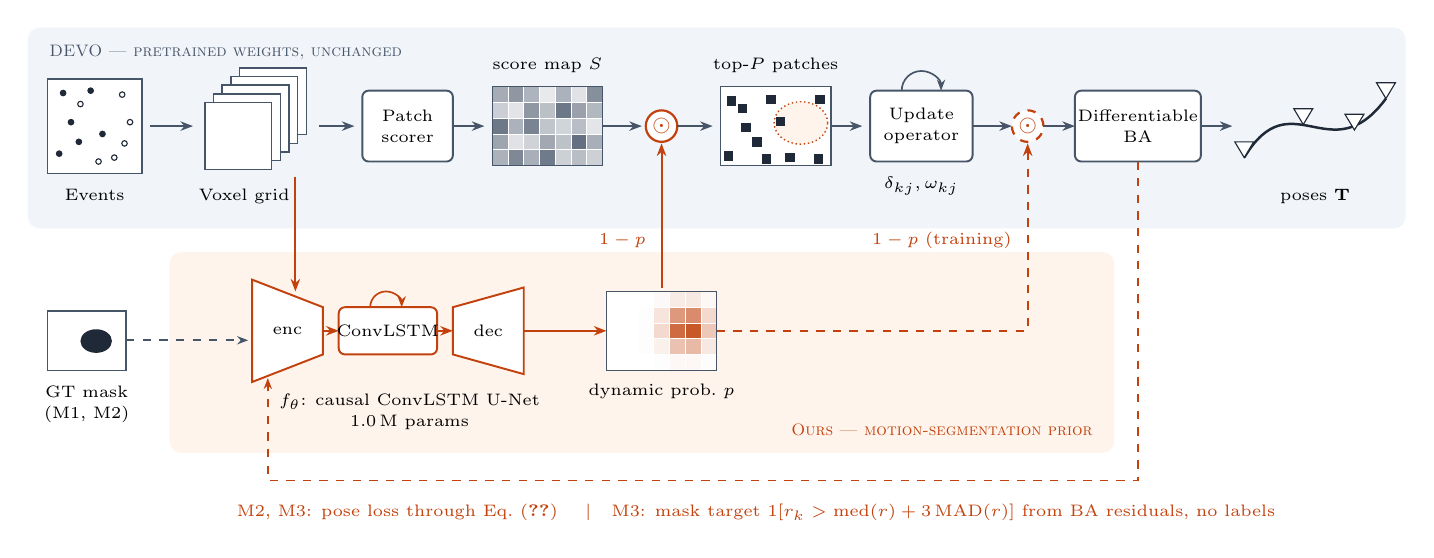
\begin{tikzpicture}[x=1cm, y=1cm, font=\fontsize{6.5}{7.5}\selectfont,
  arr/.style={-{Stealth[length=1.6mm]}, line width=0.7pt},
  box/.style={rounded corners=0.8mm, line width=0.7pt, fill=white, align=center}]
\fill[slatelight, rounded corners=1.5mm] (-0.25,-1.3) rectangle (17.25,1.25);
\node[anchor=north west, text=slate, font=\fontsize{6}{7}\selectfont] at (-0.1,1.15) {\textsc{DEVO --- pretrained weights, unchanged}};
\fill[ourslight, rounded corners=1.5mm] (1.55,-4.15) rectangle (13.55,-1.6);
\node[anchor=south east, text=ours, font=\fontsize{6}{7}\selectfont] at (13.4,-4.05) {\textsc{Ours --- motion-segmentation prior}};
\draw[slate, line width=0.5pt, fill=white] (0,-0.6) rectangle (1.2,0.6);
\draw[ink, line width=0.4pt, fill=ink] (0.15,-0.35) circle (0.035);
\draw[ink, line width=0.4pt, fill=white] (0.42,0.28) circle (0.035);
\draw[ink, line width=0.4pt, fill=ink] (0.7,-0.1) circle (0.035);
\draw[ink, line width=0.4pt, fill=white] (0.95,0.4) circle (0.035);
\draw[ink, line width=0.4pt, fill=ink] (0.3,0.05) circle (0.035);
\draw[ink, line width=0.4pt, fill=white] (0.85,-0.4) circle (0.035);
\draw[ink, line width=0.4pt, fill=ink] (0.55,0.45) circle (0.035);
\draw[ink, line width=0.4pt, fill=white] (1.05,0.05) circle (0.035);
\draw[ink, line width=0.4pt, fill=ink] (0.2,0.42) circle (0.035);
\draw[ink, line width=0.4pt, fill=white] (0.65,-0.45) circle (0.035);
\draw[ink, line width=0.4pt, fill=ink] (0.4,-0.2) circle (0.035);
\draw[ink, line width=0.4pt, fill=white] (0.98,-0.22) circle (0.035);
\node[anchor=north] at (0.6,-0.68) {Events};
\draw[arr, slate] (1.3,0) -- (1.85,0);
\draw[slate, line width=0.5pt, fill=white] (2.44,-0.11) rectangle +(0.85,0.85);
\draw[slate, line width=0.5pt, fill=white] (2.33,-0.22) rectangle +(0.85,0.85);
\draw[slate, line width=0.5pt, fill=white] (2.22,-0.33) rectangle +(0.85,0.85);
\draw[slate, line width=0.5pt, fill=white] (2.11,-0.44) rectangle +(0.85,0.85);
\draw[slate, line width=0.5pt, fill=white] (2,-0.55) rectangle +(0.85,0.85);
\node[anchor=north] at (2.5,-0.68) {Voxel grid};
\draw[arr, slate] (3.45,0) -- (3.9,0);
\draw[box, draw=slate] (4.0,-0.45) rectangle (5.15,0.45); \node[align=center] at (4.575,0) {Patch\\scorer};
\draw[arr, slate] (5.15,0) -- (5.55,0);
\fill[slate!45!white, draw=white, line width=0.25pt] (5.65,-0.5) rectangle +(0.2,0.2);
\fill[slate!53!white, draw=white, line width=0.25pt] (5.65,-0.3) rectangle +(0.2,0.2);
\fill[slate!79!white, draw=white, line width=0.25pt] (5.65,-0.1) rectangle +(0.2,0.2);
\fill[slate!28!white, draw=white, line width=0.25pt] (5.65,0.1) rectangle +(0.2,0.2);
\fill[slate!49!white, draw=white, line width=0.25pt] (5.65,0.3) rectangle +(0.2,0.2);
\fill[slate!70!white, draw=white, line width=0.25pt] (5.85,-0.5) rectangle +(0.2,0.2);
\fill[slate!17!white, draw=white, line width=0.25pt] (5.85,-0.3) rectangle +(0.2,0.2);
\fill[slate!45!white, draw=white, line width=0.25pt] (5.85,-0.1) rectangle +(0.2,0.2);
\fill[slate!16!white, draw=white, line width=0.25pt] (5.85,0.1) rectangle +(0.2,0.2);
\fill[slate!61!white, draw=white, line width=0.25pt] (5.85,0.3) rectangle +(0.2,0.2);
\fill[slate!47!white, draw=white, line width=0.25pt] (6.05,-0.5) rectangle +(0.2,0.2);
\fill[slate!26!white, draw=white, line width=0.25pt] (6.05,-0.3) rectangle +(0.2,0.2);
\fill[slate!73!white, draw=white, line width=0.25pt] (6.05,-0.1) rectangle +(0.2,0.2);
\fill[slate!61!white, draw=white, line width=0.25pt] (6.05,0.1) rectangle +(0.2,0.2);
\fill[slate!44!white, draw=white, line width=0.25pt] (6.05,0.3) rectangle +(0.2,0.2);
\fill[slate!78!white, draw=white, line width=0.25pt] (6.25,-0.5) rectangle +(0.2,0.2);
\fill[slate!51!white, draw=white, line width=0.25pt] (6.25,-0.3) rectangle +(0.2,0.2);
\fill[slate!34!white, draw=white, line width=0.25pt] (6.25,-0.1) rectangle +(0.2,0.2);
\fill[slate!37!white, draw=white, line width=0.25pt] (6.25,0.1) rectangle +(0.2,0.2);
\fill[slate!13!white, draw=white, line width=0.25pt] (6.25,0.3) rectangle +(0.2,0.2);
\fill[slate!27!white, draw=white, line width=0.25pt] (6.45,-0.5) rectangle +(0.2,0.2);
\fill[slate!36!white, draw=white, line width=0.25pt] (6.45,-0.3) rectangle +(0.2,0.2);
\fill[slate!25!white, draw=white, line width=0.25pt] (6.45,-0.1) rectangle +(0.2,0.2);
\fill[slate!80!white, draw=white, line width=0.25pt] (6.45,0.1) rectangle +(0.2,0.2);
\fill[slate!45!white, draw=white, line width=0.25pt] (6.45,0.3) rectangle +(0.2,0.2);
\fill[slate!38!white, draw=white, line width=0.25pt] (6.65,-0.5) rectangle +(0.2,0.2);
\fill[slate!84!white, draw=white, line width=0.25pt] (6.65,-0.3) rectangle +(0.2,0.2);
\fill[slate!38!white, draw=white, line width=0.25pt] (6.65,-0.1) rectangle +(0.2,0.2);
\fill[slate!55!white, draw=white, line width=0.25pt] (6.65,0.1) rectangle +(0.2,0.2);
\fill[slate!17!white, draw=white, line width=0.25pt] (6.65,0.3) rectangle +(0.2,0.2);
\fill[slate!27!white, draw=white, line width=0.25pt] (6.85,-0.5) rectangle +(0.2,0.2);
\fill[slate!47!white, draw=white, line width=0.25pt] (6.85,-0.3) rectangle +(0.2,0.2);
\fill[slate!15!white, draw=white, line width=0.25pt] (6.85,-0.1) rectangle +(0.2,0.2);
\fill[slate!42!white, draw=white, line width=0.25pt] (6.85,0.1) rectangle +(0.2,0.2);
\fill[slate!66!white, draw=white, line width=0.25pt] (6.85,0.3) rectangle +(0.2,0.2);
\draw[slate, line width=0.5pt] (5.65,-0.5) rectangle +(1.4,1);
\node[anchor=south] at (6.35,0.55) {score map $S$};
\draw[arr, slate] (7.05,0) -- (7.55,0);
\draw[ours, line width=0.8pt, fill=white] (7.8,0) circle (0.2); \node[text=ours, font=\fontsize{8}{8}\selectfont] at (7.8,0) {$\odot$};
\draw[arr, slate] (8.0,0) -- (8.45,0);
\draw[slate, line width=0.5pt, fill=white] (8.55,-0.5) rectangle +(1.4,1.0);
\draw[ours, line width=0.5pt, densely dotted, fill=ourslight] (9.57,0.04) ellipse (0.34 and 0.27);
\fill[ink] (8.59,-0.44) rectangle +(0.12,0.12);
\fill[ink] (8.77,0.16) rectangle +(0.12,0.12);
\fill[ink] (8.95,-0.26) rectangle +(0.12,0.12);
\fill[ink] (8.63,0.26) rectangle +(0.12,0.12);
\fill[ink] (9.13,0.28) rectangle +(0.12,0.12);
\fill[ink] (9.07,-0.48) rectangle +(0.12,0.12);
\fill[ink] (8.81,-0.08) rectangle +(0.12,0.12);
\fill[ink] (9.73,-0.48) rectangle +(0.12,0.12);
\fill[ink] (9.25,-0) rectangle +(0.12,0.12);
\fill[ink] (9.75,0.28) rectangle +(0.12,0.12);
\fill[ink] (9.37,-0.46) rectangle +(0.12,0.12);
\node[anchor=south] at (9.25,0.55) {top-$P$ patches};
\draw[arr, slate] (9.95,0) -- (10.35,0);
\draw[box, draw=slate] (10.45,-0.45) rectangle (11.75,0.45); \node[align=center] at (11.1,0) {Update\\operator};
\draw[slate, line width=0.6pt, -{Stealth[length=1.4mm]}] (10.85,0.45) arc[start angle=180, end angle=0, radius=0.25];
\node[anchor=north] at (11.1,-0.52) {$\delta_{kj}, \omega_{kj}$};
\draw[arr, slate] (11.75,0) -- (12.25,0);
\draw[ours, line width=0.8pt, dashed, fill=white] (12.45,0) circle (0.2); \node[text=ours, font=\fontsize{8}{8}\selectfont] at (12.45,0) {$\odot$};
\draw[arr, slate] (12.65,0) -- (13.05,0);
\draw[box, draw=slate] (13.05,-0.45) rectangle (14.65,0.45); \node[align=center] at (13.85,0) {Differentiable\\BA};
\draw[arr, slate] (14.65,0) -- (15.05,0);
\draw[ink, line width=0.9pt] (15.2,-0.4) .. controls (15.8,0.6) and (16.3,-0.6) .. (17.0,0.35);
\draw[ink, line width=0.4pt, fill=white] (15.2,-0.4) -- (15.08,-0.2) -- (15.32,-0.2) -- cycle;
\draw[ink, line width=0.4pt, fill=white] (15.95,0.02) -- (15.83,0.22) -- (16.07,0.22) -- cycle;
\draw[ink, line width=0.4pt, fill=white] (16.6,-0.05) -- (16.48,0.15) -- (16.72,0.15) -- cycle;
\draw[ink, line width=0.4pt, fill=white] (17.0,0.35) -- (16.88,0.55) -- (17.12,0.55) -- cycle;
\node[anchor=north] at (16.1,-0.68) {poses $\mathbf{T}$};
\draw[ours, line width=0.7pt, fill=white] (2.6,-3.25) -- (2.6,-1.95) -- (3.5,-2.3) -- (3.5,-2.9) -- cycle; \node at (3.05,-2.6) {enc};
\draw[box, draw=ours] (3.7,-2.9) rectangle (4.95,-2.3); \node at (4.325,-2.6) {ConvLSTM};
\draw[ours, line width=0.6pt, -{Stealth[length=1.4mm]}] (4.1,-2.3) arc[start angle=180, end angle=0, radius=0.2];
\draw[ours, line width=0.7pt, fill=white] (5.15,-2.9) -- (5.15,-2.3) -- (6.05,-2.05) -- (6.05,-3.15) -- cycle; \node at (5.6,-2.6) {dec};
\draw[arr, ours] (3.5,-2.6) -- (3.7,-2.6); \draw[arr, ours] (4.95,-2.6) -- (5.15,-2.6);
\node[anchor=north, align=center] at (4.6,-3.28) {$f_\theta$: causal ConvLSTM U-Net\\1.0\,M params};
\draw[arr, ours] (3.15,-0.65) -- (3.15,-2.1);
\draw[arr, ours] (6.05,-2.6) -- (7.1,-2.6);
\fill[ours!0!white, draw=white, line width=0.25pt] (7.1,-3.1) rectangle +(0.2,0.2);
\fill[ours!0!white, draw=white, line width=0.25pt] (7.1,-2.9) rectangle +(0.2,0.2);
\fill[ours!0!white, draw=white, line width=0.25pt] (7.1,-2.7) rectangle +(0.2,0.2);
\fill[ours!0!white, draw=white, line width=0.25pt] (7.1,-2.5) rectangle +(0.2,0.2);
\fill[ours!0!white, draw=white, line width=0.25pt] (7.1,-2.3) rectangle +(0.2,0.2);
\fill[ours!0!white, draw=white, line width=0.25pt] (7.3,-3.1) rectangle +(0.2,0.2);
\fill[ours!0!white, draw=white, line width=0.25pt] (7.3,-2.9) rectangle +(0.2,0.2);
\fill[ours!0!white, draw=white, line width=0.25pt] (7.3,-2.7) rectangle +(0.2,0.2);
\fill[ours!0!white, draw=white, line width=0.25pt] (7.3,-2.5) rectangle +(0.2,0.2);
\fill[ours!0!white, draw=white, line width=0.25pt] (7.3,-2.3) rectangle +(0.2,0.2);
\fill[ours!0!white, draw=white, line width=0.25pt] (7.5,-3.1) rectangle +(0.2,0.2);
\fill[ours!1!white, draw=white, line width=0.25pt] (7.5,-2.9) rectangle +(0.2,0.2);
\fill[ours!1!white, draw=white, line width=0.25pt] (7.5,-2.7) rectangle +(0.2,0.2);
\fill[ours!1!white, draw=white, line width=0.25pt] (7.5,-2.5) rectangle +(0.2,0.2);
\fill[ours!0!white, draw=white, line width=0.25pt] (7.5,-2.3) rectangle +(0.2,0.2);
\fill[ours!1!white, draw=white, line width=0.25pt] (7.7,-3.1) rectangle +(0.2,0.2);
\fill[ours!8!white, draw=white, line width=0.25pt] (7.7,-2.9) rectangle +(0.2,0.2);
\fill[ours!20!white, draw=white, line width=0.25pt] (7.7,-2.7) rectangle +(0.2,0.2);
\fill[ours!14!white, draw=white, line width=0.25pt] (7.7,-2.5) rectangle +(0.2,0.2);
\fill[ours!3!white, draw=white, line width=0.25pt] (7.7,-2.3) rectangle +(0.2,0.2);
\fill[ours!4!white, draw=white, line width=0.25pt] (7.9,-3.1) rectangle +(0.2,0.2);
\fill[ours!32!white, draw=white, line width=0.25pt] (7.9,-2.9) rectangle +(0.2,0.2);
\fill[ours!78!white, draw=white, line width=0.25pt] (7.9,-2.7) rectangle +(0.2,0.2);
\fill[ours!54!white, draw=white, line width=0.25pt] (7.9,-2.5) rectangle +(0.2,0.2);
\fill[ours!11!white, draw=white, line width=0.25pt] (7.9,-2.3) rectangle +(0.2,0.2);
\fill[ours!4!white, draw=white, line width=0.25pt] (8.1,-3.1) rectangle +(0.2,0.2);
\fill[ours!37!white, draw=white, line width=0.25pt] (8.1,-2.9) rectangle +(0.2,0.2);
\fill[ours!88!white, draw=white, line width=0.25pt] (8.1,-2.7) rectangle +(0.2,0.2);
\fill[ours!61!white, draw=white, line width=0.25pt] (8.1,-2.5) rectangle +(0.2,0.2);
\fill[ours!12!white, draw=white, line width=0.25pt] (8.1,-2.3) rectangle +(0.2,0.2);
\fill[ours!1!white, draw=white, line width=0.25pt] (8.3,-3.1) rectangle +(0.2,0.2);
\fill[ours!12!white, draw=white, line width=0.25pt] (8.3,-2.9) rectangle +(0.2,0.2);
\fill[ours!29!white, draw=white, line width=0.25pt] (8.3,-2.7) rectangle +(0.2,0.2);
\fill[ours!20!white, draw=white, line width=0.25pt] (8.3,-2.5) rectangle +(0.2,0.2);
\fill[ours!4!white, draw=white, line width=0.25pt] (8.3,-2.3) rectangle +(0.2,0.2);
\draw[slate, line width=0.5pt] (7.1,-3.1) rectangle +(1.4,1);
\node[anchor=north] at (7.8,-3.15) {dynamic prob.\ $p$};
\draw[arr, ours] (7.8,-2.05) -- (7.8,-0.22); \node[anchor=east, text=ours] at (7.72,-1.45) {$1-p$};
\draw[arr, ours, dashed] (8.5,-2.6) -- (12.45,-2.6) -- (12.45,-0.22); \node[anchor=east, text=ours] at (12.37,-1.45) {$1-p$ (training)};
\draw[slate, line width=0.5pt, fill=white] (0,-3.1) rectangle +(1.0,0.75); \fill[ink] (0.62,-2.73) ellipse (0.2 and 0.15);
\node[anchor=north, align=center] at (0.5,-3.18) {GT mask\\(M1, M2)};
\draw[slate, line width=0.6pt, dashed, -{Stealth[length=1.4mm]}] (1.0,-2.72) -- (2.55,-2.72);
\draw[ours, line width=0.6pt, dashed, -{Stealth[length=1.4mm]}] (13.85,-0.45) -- (13.85,-4.5) -- (2.8,-4.5) -- (2.8,-3.2);
\node[anchor=north, text=ours] at (9.0,-4.68) {M2, M3: pose loss through Eq.~\eqref{eq:inject} \quad$|$\quad M3: mask target $\mathbb{1}[r_k > \mathrm{med}(r) + 3\,\mathrm{MAD}(r)]$ from BA residuals, no labels};
\end{tikzpicture}
}
\caption{Overview. Gray: DEVO~\cite{klenk2024devo}, unchanged (events are binned into a
voxel grid of $B = 5$ temporal bins). Orange: our additions. A causal network $f_\theta$
predicts the probability $p$ that each score-map cell belongs to a moving object; $1 - p$
attenuates the patch-selection score $S$ (solid, used at training and inference) and the
BA confidences $\omega_{kj}$ (dashed, coupled training only), \cref{eq:inject}. Dashed
arrows at the bottom are training signals: ground-truth masks (M1, M2), pose loss (M2, M3)
and bundle-adjustment residual outliers (M3).}
\label{fig:arch}
\end{figure*}

\subsection{Three ways to train the predictor}

All variants share the predictor architecture and the injection \cref{eq:inject}; they
differ only in how $f_\theta$ (and possibly DEVO) is trained.

\textbf{M1 --- decoupled (plug-in).} $f_\theta$ is trained alone on ground-truth masks
with a binary cross-entropy plus Dice loss (weight 0.5), the positive class weighted by a
factor $\wplus$. DEVO keeps its public pretrained weights. This is the ``beside'' option.

\textbf{M2 --- coupled, supervised.} $f_\theta$ is initialized from M1 and trained jointly
with DEVO: the total loss is DEVO's pose and flow loss plus a weighted BCE between $p$ and
the ground-truth mask,
$\mathcal{L} = \mathcal{L}_\text{pose} + \lambda \mathcal{L}_\text{mask}$ with
$\lambda = 1$. The pose gradient flows through \cref{eq:inject} into $\theta$.

\textbf{M3 --- coupled, self-supervised.} Same as M2, but the mask target comes from the
DBA instead of annotations. For each patch $k$ we compute the mean, over its edges, of the
residual $r_k$ between the update operator's target and the reprojection under the
estimated pose, and flag outliers with a robust threshold:
\begin{equation}
\tilde{y}_k = \mathbb{1}\left[r_k > \mathrm{med}(r) + 3 \cdot \mathrm{MAD}(r)\right].
\label{eq:selfsup}
\end{equation}
$\mathcal{L}_\text{mask}$ is then the BCE between $p(\mathbf{P}_k)$ and $\tilde{y}_k$. No
ground-truth mask enters the loss. DEVO's own score loss uses the same kind of signal,
residuals weighted by confidence, without labels~\cite{klenk2024devo}; we redirect it from
``is this patch trackable?'' to ``is this patch rigid?''.

For both coupled variants we also train \emph{scratch} versions in which $f_\theta$ is
randomly initialized, with a soft prior $\beta (\bar{p} - 0.02)^2$, $\beta = 0.5$, that
keeps the mean mask near the true positive rate and prevents collapse.

\textbf{Control --- DEVO-ft.} To separate the effect of the mask from that of adapting DEVO
to EVIMO2, we fine-tune DEVO on exactly the same data and schedule with the mask set to
zero. This control turns out to be decisive (\cref{sec:results}).

\subsection{Ground-truth dynamic masks}

EVIMO2~\cite{burner2022evimo2} provides per-pixel masks of every object tracked by motion
capture, including objects that never move. Taking ``mask $\neq 0$'' as the target (the
definition we used initially, called \code{all} below) labels 61\% of score-map cells as
dynamic on the training split, and the corresponding oracle mostly removes static
scenery. We instead reconstruct each object's world trajectory from the motion-capture
poses and label an object as dynamic at time $t$ if it deviates by more than 1\,cm from
its median position over $[t - 0.1, t + 0.1]$\,s, an effective speed threshold of about
10\,cm/s. The 1\,cm threshold is 1.5 times the largest window deviation measured on static
objects (0.66\,cm, pose noise); the 0.2\,s window keeps the label close to causal. With
this definition, 1.9\% of training cells are positive and 66\% of training frames contain
no moving object. Masks are dilated by 1\,px, identically for training, for M2 supervision
and for the oracle. Since the class ratio is about 1:50, we use
$\wplus = 7 \approx \sqrt{50}$ by default and select $\wplus = 3$ by a sweep over
$\{3, 7, 15\}$ on three sequences held out from the training split; we report both.

% ======================================================================================
\section{Experimental Setup}

\textbf{Data.} Training uses the 21 sequences of the EVIMO2 IMO training split (Samsung
mono camera, $640 \times 480$, 4,745 frames). Evaluation uses the 8 sequences of the IMO
evaluation split, disjoint from training. For cross-dataset evaluation we run every model,
trained on EVIMO2 only, on the sequences used by DEVO~\cite{klenk2024devo}: RPG stereo
(8)~\cite{zhou2018semidense}, MVSEC indoor flying (4)~\cite{zhu2018mvsec},
EDS (9)~\cite{hidalgo2022eds}, VECtor (17)~\cite{gao2022vector} and TUM-VIE (5
motion-capture sequences)~\cite{klenk2021tumvie}. These are mostly static scenes: they
measure out-of-domain robustness, not the benefit of the mask.

\textbf{Training.} M1: 100 epochs, AdamW, learning rate $10^{-3}$ with cosine decay,
batches of 8 clips of 16 frames. We keep the checkpoint with the best validation IoU
(\code{best\_iou.pt}). Coupled variants: 40k steps on clips of 15 frames, DEVO frozen for
the first 10k steps (only $f_\theta$ adapts), then both trained with learning rates
$10^{-4}$ ($f_\theta$) and $2 \cdot 10^{-5}$ (DEVO), gradient clipping at 10. DEVO-ft: the
30k unfrozen steps of the same schedule. Every configuration is trained with 5 seeds.

\textbf{Evaluation.} We report the absolute trajectory error (ATE, translation, in cm)
after Sim(3) alignment, as DEVO does. DEVO samples patches stochastically, so each sequence
is run 10 times; a seed's score is the mean over sequences of the mean over trials, and
tables report mean $\pm$ standard deviation \emph{across the 5 training seeds} (the
evaluation seed equals the training seed). For cross-dataset tables, where a few divergent
runs can dominate a mean, we report the mean over sequences of the per-sequence median over
all trials, and the share of failed trials (ATE $>$ 50\,cm; $>$ 10\,cm on TUM-VIE). The
oracle replaces $p$ by the ground-truth dynamic mask.

% ======================================================================================
\section{Results}\label{sec:results}

\subsection{Pretrained DEVO: a plug-in mask matches the oracle}

\begin{table}[t]
\centering
\caption{EVIMO2, 8 evaluation sequences, DEVO with its public weights. Mean $\pm$ std
over 5 training seeds (10 trials per sequence and seed).}
\label{tab:pretrained}
\begin{tabular}{lcc}
\toprule
Method (DEVO weights: pretrained) & ATE (cm) $\downarrow$ & $\Delta$ vs.\ DEVO \\
\midrule
DEVO~\cite{klenk2024devo} & \pmstd{2.08}{0.18} & -- \\
+ oracle (GT dynamic mask) & \pmstd{1.70}{0.22} & $-18\%$ \\
\midrule
+ M1, $\wplus = 7$ & \pmstd{1.94}{0.14} & $-7\%$ \\
+ M1, $\wplus = 3$ & \pmstd{\best{1.72}}{0.29} & \best{$-17\%$} \\
+ M1, $\wplus = 7$, last checkpoint & \pmstd{1.80}{0.14} & $-13\%$ \\
+ M1, $\wplus = 3$, last checkpoint & \pmstd{1.76}{0.14} & $-15\%$ \\
+ M1, $D = 128$, $\wplus = 7$ & \pmstd{1.90}{0.16} & $-9\%$ \\
\bottomrule
\end{tabular}
\end{table}

\Cref{tab:pretrained} shows that motion awareness helps a pretrained DEVO. The oracle
lowers the ATE by 18\%, which bounds what a mask can bring through the score map on these
sequences; it is much less than the 41\% we measured during the project with the
\code{all} mask definition, most of which came from masking static scenery
(\cref{sec:all}). The plug-in predictor with $\wplus = 3$ reaches 1.72\,cm, within noise
of the oracle. Lower positive weights help: a strong recall bias ($\wplus = 7$) masks too
much of the image. A larger predictor ($D = 128$) brings nothing.

These gains must be read with their uncertainty. The oracle improves on DEVO for all 5
seeds, but the plug-in predictor ($\wplus = 3$) for 4 of 5; a Wilcoxon signed-rank test
over the 40 (seed, sequence) pairs gives $p = 0.051$ for the oracle and $p = 0.24$ for M1
($p = 0.77$ for $\wplus = 7$). On 8 sequences, the improvement of M1 is consistent in
direction but not statistically significant.

\code{best\_iou.pt} is selected on the evaluation split, which biases M1 favorably. The
last checkpoint, which involves no selection, gives 1.76\,cm ($\wplus = 3$) and 1.80\,cm
($\wplus = 7$): the bias is small and the conclusion unchanged. As a segmenter, M1 is
modest: its best validation IoU against the motion-based ground truth, at score-map
resolution, is $0.36 \pm 0.02$ ($\wplus = 3$), $0.35 \pm 0.02$ ($\wplus = 7$) and
$0.26 \pm 0.01$ ($D = 128$). Trained on the \code{all} definition, the same network reaches
$0.93$: recognizing motion-captured props is easy, detecting which of them move from
events alone is not. A mask of IoU 0.36 is nevertheless enough to recover most of the
oracle's gain, because the score map only needs to steer patches away from moving regions,
not to delineate them. Over the 8 sequences, 5.4\% of the patches selected by DEVO fall on
cells that the ground truth labels as moving; M1 halves this share (2.7\%) and the oracle
brings it to 0.7\% (\cref{fig:patches} in the supplementary material).

The gain is concentrated on a few sequences (\cref{tab:perscene}). Four of the eight
sequences account for 89\% of DEVO's error, and the largest improvement comes from
\code{scene14\_dyn\_test\_04} (5.11 $\to$ 3.60\,cm with the oracle) and
\code{scene14\_dyn\_test\_05} (2.38 $\to$ 1.46\,cm with M1). With only 8 evaluation
sequences, the per-sequence variance is large, which is why we average over seeds and
trials.

\subsection{Joint training: the gain is domain adaptation}

\begin{table*}[t]
\centering
\caption{EVIMO2 ATE (cm), models whose DEVO weights were fine-tuned on EVIMO2. Each M2/M3
cell uses its own jointly trained weights; ``oracle'' and ``M1'' rows use the DEVO-ft
weights. Mean $\pm$ std over 5 seeds. For comparison, pretrained DEVO: 2.08.}
\label{tab:finetuned}
\begin{tabular}{lcccc}
\toprule
DEVO fine-tuned on EVIMO2 & $\wplus = 7$ & $\wplus = 3$ & scratch & $D = 128$ \\
\midrule
DEVO-ft (no mask) & \multicolumn{4}{c}{\pmstd{1.20}{0.16}} \\
+ oracle & \multicolumn{4}{c}{\pmstd{1.27}{0.15}} \\
+ M1 & \multicolumn{4}{c}{\pmstd{1.35}{0.12}} \\
\midrule
M2 (coupled, GT) & \pmstd{1.39}{0.19} & \pmstd{1.19}{0.13} & \pmstd{1.34}{0.07} & \pmstd{1.04}{0.28} \\
M3 (coupled, residual) & \pmstd{1.48}{0.22} & \pmstd{1.26}{0.21} & \pmstd{1.61}{0.50} & \pmstd{1.22}{0.50} \\
\bottomrule
\end{tabular}
\end{table*}

Coupled models reach much lower errors than pretrained DEVO (\cref{tab:finetuned}):
1.19\,cm for M2 and 1.26\,cm for M3 with $\wplus = 3$, about 40\% below DEVO. Read alone,
this would suggest that joint training is the right design. The DEVO-ft control rules this
out: fine-tuning DEVO on the same data, with the same schedule and no mask at all, gives
1.20\,cm, the level of the best coupled model. Once DEVO is fine-tuned, the mask no longer
helps: the oracle gives 1.27\,cm and M1 1.35\,cm on top of DEVO-ft, both within noise of,
or slightly worse than, DEVO-ft alone. The per-sequence view confirms it
(\cref{tab:perscene}): fine-tuning alone brings \code{scene14\_dyn\_test\_04} from 5.11 to
0.25\,cm, far beyond what the oracle mask achieves on pretrained DEVO.

Our interpretation is that the fine-tuned DEVO has learned EVIMO2's statistics (sensor,
event rate, motion range, scene layout) well enough to discount the moving objects of this
dataset on its own, through its update operator and confidences. The only coupled
configuration below DEVO-ft is M2 with $D = 128$ (1.04\,cm), but its seed variance (0.28)
makes the difference with DEVO-ft ($1.20 \pm 0.16$) inconclusive: it wins on 3 of 5 seeds,
and a Wilcoxon test over the 40 (seed, sequence) pairs gives $p = 0.31$ ($p = 0.44$ for M2
with $\wplus = 3$, $p = 0.58$ for M3 with $D = 128$). No coupled variant is significantly
different from DEVO-ft.

Self-supervision from DBA residuals (M3) trains a usable mask: with the same
initialization it stays within 0.1\,cm of mask-supervised M2 ($\wplus = 3$: 1.26 vs.\
1.19), and from scratch within 0.3\,cm (1.61 vs.\ 1.34), with larger seed variance. The
residual is therefore a viable label-free signal, but on EVIMO2 it is not a better one than
ground truth, contrary to what our earlier single-seed experiments suggested.

\subsection{Generalization: fine-tuning on EVIMO2 does not transfer}

\begin{table*}[t]
\centering
\caption{Cross-dataset ATE (cm), all models trained on EVIMO2 only. Mean over sequences of
the per-sequence median over all trials; in parentheses, share of failed trials
($>$ 50\,cm, $>$ 10\,cm on TUM-VIE). Number of sequences in the header. Between 5 and 101
evaluation runs per cell, 3--10 trials each (see supplementary).}
\label{tab:cross}
\begin{tabular}{lccccc}
\toprule
Method & RPG (8) & MVSEC (4) & EDS (9) & VECtor (17) & TUM-VIE (5) \\
\midrule
DEVO (pretrained) & 1.0 (0\%) & 13.7 (17\%) & 33.8 (16\%) & 55.1 (28\%) & \best{1.2} (0\%) \\
+ M1, $\wplus = 3$ & 1.0 (0\%) & 13.8 (\best{13\%}) & \best{31.4} (22\%) & \best{50.6} (29\%) & 1.5 (0\%) \\
+ M1, $\wplus = 7$ & 1.0 (0\%) & 13.9 (15\%) & 38.7 (26\%) & 54.0 (31\%) & 1.3 (0\%) \\
+ M1, \code{all} mask & 1.0 (0\%) & 16.9 (16\%) & 43.8 (33\%) & 57.7 (32\%) & 1.2 (1\%) \\
\midrule
DEVO-ft & 2.7 (0\%) & 49.1 (39\%) & 127.0 (97\%) & 415 (35\%) & 11.5 (57\%) \\
M2, $\wplus = 7$ / 3 & 3.0 / 2.7 & 45.5 / 43.4 & 126.8 / 121.1 & 435 / 393 & 11.9 / 11.4 \\
M3, $\wplus = 7$ / 3 & 2.5 / 2.5 & 47.4 / 43.3 & 116.8 / 127.8 & 399 / 442 & 11.3 / 11.1 \\
M1 on DEVO-ft & 2.8 & 52.4 & 127.2 & 417 & 13.4 \\
\bottomrule
\end{tabular}
\end{table*}

\Cref{tab:cross,fig:ratio} show the price of fine-tuning. Every model whose DEVO weights
were trained on EVIMO2 (DEVO-ft, all M2 and M3 variants, M1 on DEVO-ft) degrades sharply
outside EVIMO2, regardless of the mask: about $\times 3$ on RPG and MVSEC, $\times 4$ on
EDS (97\% failed trials), $\times 7$ on VECtor and $\times 9$ on TUM-VIE. Twenty-one EVIMO2
training sequences are far too few to keep the generality DEVO acquired on synthetic
TartanAir data, and the coupled models inherit this overfitting from their DEVO part.

The plug-in predictor (M1) leaves DEVO's weights untouched, and keeps its generalization:
it is on par with DEVO on RPG, MVSEC and TUM-VIE, slightly better on VECtor (50.6 vs.\
55.1\,cm) and on the failure rate of MVSEC (13\% vs.\ 17\%), and mixed on EDS (lower median
error but more failures). EDS illustrates the remaining risk of the plug-in approach: the
EVIMO2-trained predictor flags 11--35\% of the image as moving on EDS sequences, against
1--9\% on RPG and MVSEC, so it removes useful static structure on a dataset whose texture
and motion statistics it has never seen (\cref{fig:patches}). Sharpening the mask does not
remove this risk (\cref{sec:variants}).

\begin{figure}[t]
\centering
\resizebox{\columnwidth}{!}{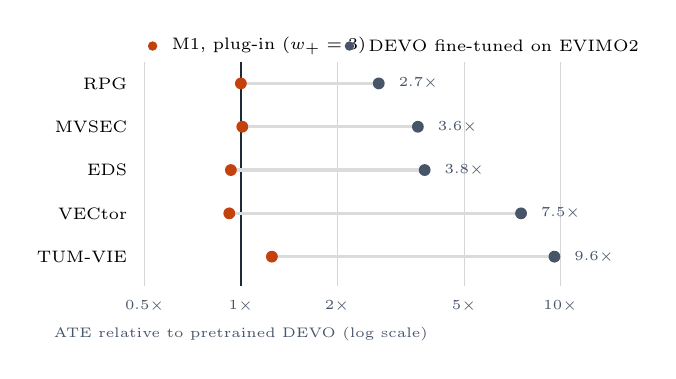
\begin{tikzpicture}[x=1cm, y=1cm, font=\fontsize{6.5}{7.5}\selectfont]
\draw[black!16, line width=0.4pt] (0,-0.1) -- (0,2.75);
\node[anchor=north, text=slate, font=\fontsize{5.5}{6.5}\selectfont] at (0,-0.15) {0.5$\times$};
\draw[ink, line width=0.6pt] (1.221,-0.1) -- (1.221,2.75);
\node[anchor=north, text=slate, font=\fontsize{5.5}{6.5}\selectfont] at (1.221,-0.15) {1$\times$};
\draw[black!16, line width=0.4pt] (2.443,-0.1) -- (2.443,2.75);
\node[anchor=north, text=slate, font=\fontsize{5.5}{6.5}\selectfont] at (2.443,-0.15) {2$\times$};
\draw[black!16, line width=0.4pt] (4.057,-0.1) -- (4.057,2.75);
\node[anchor=north, text=slate, font=\fontsize{5.5}{6.5}\selectfont] at (4.057,-0.15) {5$\times$};
\draw[black!16, line width=0.4pt] (5.279,-0.1) -- (5.279,2.75);
\node[anchor=north, text=slate, font=\fontsize{5.5}{6.5}\selectfont] at (5.279,-0.15) {10$\times$};
\node[anchor=east] at (-0.1,2.475) {RPG};
\draw[black!14, line width=1.2pt] (1.221,2.475) -- (2.972,2.475);
\fill[slate] (2.972,2.475) circle (0.075); \fill[ours] (1.221,2.475) circle (0.075);
\node[anchor=west, text=slate, font=\fontsize{5.5}{6.5}\selectfont] at (3.102,2.475) {2.7$\times$};
\node[anchor=east] at (-0.1,1.925) {MVSEC};
\draw[black!14, line width=1.2pt] (1.239,1.925) -- (3.469,1.925);
\fill[slate] (3.469,1.925) circle (0.075); \fill[ours] (1.239,1.925) circle (0.075);
\node[anchor=west, text=slate, font=\fontsize{5.5}{6.5}\selectfont] at (3.599,1.925) {3.6$\times$};
\node[anchor=east] at (-0.1,1.375) {EDS};
\draw[black!14, line width=1.2pt] (1.094,1.375) -- (3.555,1.375);
\fill[slate] (3.555,1.375) circle (0.075); \fill[ours] (1.094,1.375) circle (0.075);
\node[anchor=west, text=slate, font=\fontsize{5.5}{6.5}\selectfont] at (3.685,1.375) {3.8$\times$};
\node[anchor=east] at (-0.1,0.825) {VECtor};
\draw[black!14, line width=1.2pt] (1.074,0.825) -- (4.779,0.825);
\fill[slate] (4.779,0.825) circle (0.075); \fill[ours] (1.074,0.825) circle (0.075);
\node[anchor=west, text=slate, font=\fontsize{5.5}{6.5}\selectfont] at (4.909,0.825) {7.5$\times$};
\node[anchor=east] at (-0.1,0.275) {TUM-VIE};
\draw[black!14, line width=1.2pt] (1.615,0.275) -- (5.203,0.275);
\fill[slate] (5.203,0.275) circle (0.075); \fill[ours] (1.615,0.275) circle (0.075);
\node[anchor=west, text=slate, font=\fontsize{5.5}{6.5}\selectfont] at (5.333,0.275) {9.6$\times$};
\node[anchor=north, text=slate, font=\fontsize{5.5}{6.5}\selectfont] at (1.221,-0.5) {ATE relative to pretrained DEVO (log scale)};
\fill[ours] (0.1,2.95) circle (0.06); \node[anchor=west, font=\fontsize{6}{7}\selectfont] at (0.22,2.95) {M1, plug-in ($w_+ = 3$)};
\fill[slate] (2.6,2.95) circle (0.06); \node[anchor=west, font=\fontsize{6}{7}\selectfont] at (2.72,2.95) {DEVO fine-tuned on EVIMO2};
\end{tikzpicture}
}
\caption{Cross-dataset ATE relative to pretrained DEVO (log scale; values of
\cref{tab:cross}). The plug-in predictor stays at $\times 1$; fine-tuning DEVO on EVIMO2
costs $\times 2.7$ to $\times 9.6$.}
\label{fig:ratio}
\end{figure}

\subsection{Alternative injections}\label{sec:variants}

\begin{table*}[t]
\centering
\caption{Variants of the injection, all on pretrained DEVO weights, $\wplus = 3$. EVIMO2:
ATE (cm), mean $\pm$ std over 5 seeds, as in \cref{tab:pretrained}. Other datasets: as in
\cref{tab:cross} (mean of per-sequence medians, share of failed trials), 5 seeds of 3--10
trials each. ``Delete events'': voxels zeroed where $p > 0.5$, score map untouched. Oracle
rows need ground-truth masks, available on EVIMO2 only; the $\omega$ variant was run on
EVIMO2 only. $^\dagger$4 seeds.}
\label{tab:variants}
\begin{tabular}{lcccccc}
\toprule
DEVO pretrained, mask from & EVIMO2 (8) & RPG (8) & MVSEC (4) & EDS (9) & VECtor (17) & TUM-VIE (5) \\
\midrule
none (DEVO) & \pmstd{2.08}{0.18} & 1.0 (0\%) & 13.7 (17\%) & 33.8 (16\%) & 55.1 (28\%) & 1.2 (0\%) \\
\midrule
M1, $S \odot (1 - p)$ (default) & \pmstd{1.72}{0.29} & 1.0 (0\%) & 13.8 (13\%) & 31.4 (22\%) & \best{50.6} (29\%) & 1.5 (0\%) \\
M1, $S$ and $\omega$ & \pmstd{1.81}{0.14} & -- & -- & -- & -- & -- \\
M1, $p^2$ & \pmstd{1.82}{0.10} & 1.0 (0\%) & \best{13.5} (13\%) & 36.2 (24\%) & 52.3 (27\%) & 1.2 (0\%) \\
M1, $p^4$ & \pmstd{1.83}{0.07} & 1.0 (0\%) & 14.7 (16\%) & 32.4 (20\%) & 59.5$^\dagger$ (20\%) & 1.2 (0\%) \\
M1, delete events & \pmstd{1.52}{0.23} & 1.0 (0\%) & 14.0 (12\%) & 72.6 (67\%) & 144.7 (28\%) & 4.2 (21\%) \\
\midrule
oracle, $S \odot (1 - p)$ (default) & \pmstd{1.70}{0.22} & -- & -- & -- & -- & -- \\
oracle, $S$ and $\omega$ & \pmstd{1.77}{0.15} & -- & -- & -- & -- & -- \\
oracle, delete events & \pmstd{\best{1.34}}{0.34} & -- & -- & -- & -- & -- \\
\midrule
M2, DEVO frozen (step 8k) & \pmstd{1.91}{0.08} & 1.0 (0\%) & 13.9 (16\%) & 39.5 (27\%) & 77.2 (28\%) & 1.5 (4\%) \\
M3, DEVO frozen (step 8k) & \pmstd{2.01}{0.06} & 1.0 (0\%) & 15.0 (20\%) & \best{26.3} (14\%) & 59.0 (21\%) & 1.2 (0\%) \\
\bottomrule
\end{tabular}
\end{table*}

\Cref{tab:variants} tests the design choices of \cref{eq:inject}, with the same
checkpoints and seeds as the main tables.

\textbf{Confidence hook at inference.} Adding the factor
$\omega_{kj} \cdot (1 - p(\mathbf{P}_k))$ in DEVO's bundle adjustment at inference changes
nothing measurable: 1.81\,cm for M1 and 1.77\,cm for the oracle, against 1.72 and 1.70
with the score map alone (Wilcoxon $p > 0.79$), and the coupled models stay within
0.06\,cm of \cref{tab:finetuned}. Once the score map has steered patches away from moving
objects, the few that remain carry little weight in the optimization.

\textbf{Temperature.} Raising $p$ to a power $\gamma$ suppresses weak detections and keeps
strong ones. It leaves EVIMO2 unchanged (1.82 and 1.83\,cm) and does not repair EDS:
$\gamma = 2$ and $\gamma = 4$ give 36.2 and 32.4\,cm with 24\% and 20\% failed trials,
against 31.4\,cm and 22\% for $\gamma = 1$. Elsewhere it stays at the level of DEVO and
M1, without a consistent direction (MVSEC 13.5 and 14.7\,cm, VECtor 52.3 and 59.5\,cm).
The false positives of \cref{fig:patches} are confident, not marginal, so a sharper mask
removes as much static structure as the original one.

\textbf{Deleting events.} Zeroing the voxels where $p > 0.5$, the upstream filtering
of~\cite{pellerito2026suppression} approximated with our mask, is the strongest variant on
EVIMO2: 1.34\,cm with the oracle ($-36\%$ vs.\ DEVO; better than the soft oracle on all 5
seeds, $p = 0.053$) and 1.52\,cm with M1 ($-27\%$, not significantly different from the
soft M1, $p = 0.60$). Most of this gain comes from one sequence,
\code{scene15\_dyn\_test\_01}, which the score-map hook leaves at 3.7\,cm and deletion
brings to 1.3--1.6\,cm; presumably the moving object there also corrupts the features of
nearby patches, which only deletion removes. The price is paid out of domain: where the
flagged regions are static, deletion removes the events DEVO needs. The error doubles on
EDS (72.6\,cm, 67\% failed trials, against 31.4\,cm and 22\% for soft M1) and nearly
triples on VECtor (144.7 vs.\ 50.6\,cm) and TUM-VIE (4.2 vs.\ 1.5\,cm, 21\% failed trials
against none); only RPG and MVSEC, where M1 flags little, are unaffected. Soft injection is
the conservative choice when the mask may be wrong; hard deletion pays off only when it is
right.

\subsection{What the mask learns: the \code{all} ablation}\label{sec:all}

With the \code{all} definition (every motion-captured object is ``dynamic''), the oracle
gives $1.54 \pm 0.19$\,cm on pretrained DEVO, and the learned M1 $0.88 \pm 0.21$\,cm,
i.e.\ $-58\%$ and better than its own oracle. This is not a motion-segmentation result. On
EVIMO2, motion-captured objects are textured props placed close to the camera, and masking
them, moving or not, also removes regions where DEVO's patches are poorly constrained; the
learned mask, being soft and spatially smooth, removes them more gracefully than the binary
oracle. The effect is specific to EVIMO2's scene layout: the same model is the worst M1
variant on MVSEC, EDS and VECtor (\cref{tab:cross}), and the \code{all} mask is
catastrophic for joint training (M2: $3.95 \pm 1.00$\,cm). We report it to show how
strongly the mask definition shapes conclusions on this dataset, and because our earlier,
single-seed results (41\% gain of the oracle) were obtained with it.

\subsection{Computational cost}

\begin{table}[t]
\centering
\caption{Compute per frame, in GFLOPs (network FLOPs; DEVO's custom CUDA kernels not
counted), with the evaluation settings ($P = 96$).}
\label{tab:cost}
\begin{tabular}{lccc}
\toprule
Resolution & MS & DEVO & Overhead \\
\midrule
$240\times180$ (RPG) & 2.5 & 54.5 & +5\% \\
$346\times260$ (MVSEC) & 5.2 & 53.7 & +10\% \\
$640\times480$ (EVIMO2) & 17.5 & 74.5 & +23\% \\
$1280\times720$ (TUM-VIE) & 52.4 & 132.7 & +39\% \\
\bottomrule
\end{tabular}
\end{table}

The predictor has 1.0\,M parameters (1.9\,MB in fp16) and needs less than 50\,MB of
activations at $640 \times 480$. Its cost is linear in the number of pixels and stays 2.5
to 22 times below DEVO's (\cref{tab:cost}), so DEVO, not the mask, decides whether the
system fits on an embedded platform. On an idle RTX 4000 Ada, the predictor takes 2.0\,ms
per $640 \times 480$ frame (0.5\,ms at $240 \times 180$, 7.3\,ms at $1280 \times 720$),
against 16--23\,ms per frame for DEVO on the same GPU, i.e.\ about 11\% added latency at
$640 \times 480$; on 4 CPU threads it takes 39\,ms. Since the mask changes slowly, it could
also run at a lower rate than DEVO.

% ======================================================================================
\section{Discussion and Limitations}

\textbf{Why the plug-in wins.} The coupled variants were meant to let the odometry decide
what to suppress. In practice, with 21 training sequences, the dominant effect of opening
DEVO's weights is adaptation to EVIMO2, which both solves the in-domain problem without
the mask and destroys out-of-domain accuracy. A coupled scheme that keeps DEVO frozen and
trains only $f_\theta$ through \cref{eq:inject} would isolate the gradient-coupling effect
without the overfitting; our schedule contains this phase (the first 10k steps). Evaluated
at step 8000, where DEVO still has its pretrained weights and $f_\theta$ has been trained
from M1 through \cref{eq:inject}, the coupled predictors keep most of DEVO's generalization
(\cref{tab:variants}): M3 stays within 10\% of DEVO on every dataset and is better on EDS
(26.3 vs.\ 33.8\,cm, the best value we measured there); M2 is worse on EDS and VECtor
(39.5 and 77.2\,cm, against 33.8 and 55.1), but far from the $\times 3$ to $\times 10$ of
the fully coupled models. In domain, however, they do not improve on the M1 they start
from: with $\wplus = 3$, M2 and M3 reach 1.91 and 2.01\,cm, against 1.72\,cm for M1. With
$\wplus = 7$, M2 improves its M1 initialization on all 5 seeds (1.53 vs.\ 1.94\,cm,
Wilcoxon $p = 0.12$) and M3 does not (2.01\,cm). The pose gradient is thus a weak and
inconsistent training signal for the mask over 8k steps; in our setting, keeping DEVO
frozen avoids the overfitting but brings no reliable gain over training the mask apart.
Note that during coupled training the pose loss reaches $\theta$ mainly through the
confidence factor, which our evaluation uses only in \cref{sec:variants}.

\textbf{Limitations.} (i) EVIMO2 is small: 8 evaluation sequences, four of which dominate
the error; conclusions rest on the seed and trial averaging. (ii) The cross-dataset
benchmarks are mostly static, so they test robustness, not dynamic-object handling; a
dynamic event dataset with ground-truth poses but no masks, where M1 and M3 could be
compared at no annotation cost, is missing. (iii) In \cref{sec:variants}, $\gamma$ and the
deletion threshold were not tuned, and the $\omega$ variant was evaluated on EVIMO2 only.
(iv) Our upstream-deletion baseline uses our mask, not the dense model
of~\cite{pellerito2026suppression}, and its frame-and-event odometry is not evaluated.
(v) Some TUM-VIE sequences (running, skating, office maze, shake) make every method fail
and are excluded from \cref{tab:cross}; the supplementary material lists them.

\textbf{Reproducibility.} While preparing this paper, we found and fixed several
evaluation bugs in our internship code that affected earlier numbers: EVIMO2 events loaded
at EVIMO1 resolution (75\% of events ignored by the mask), ATE means that included
aggregate keys (absolute errors underestimated by about 20\%), ground-truth masks paired
with the wrong frames (33\% misaligned, up to 233\,ms), and a cross-dataset loader that
silently fell back to no mask. All numbers in this paper come from the corrected code, with
one manifest per evaluation recording the exact checkpoints used.

% ======================================================================================
\section{Conclusion}

We studied where motion awareness should be added to a learned event-only odometry. A
small causal motion-segmentation network, trained on its own and plugged into DEVO's patch
selection, brings pretrained DEVO to the level of a ground-truth oracle on EVIMO2 (17\%
lower mean ATE, consistent across seeds though not significant on 8 sequences), at
5--23\% extra compute, and keeps DEVO's generalization across five other datasets.
Training the mask jointly with the odometry, with ground-truth or bundle-adjustment
supervision, gives lower in-domain errors, but a fine-tuning control shows that this comes
from adapting DEVO to EVIMO2, and the adaptation multiplies the error by up to ten
elsewhere. Until event datasets with moving objects are large and diverse enough to
fine-tune a learned odometry without overfitting, motion awareness is best kept beside the
odometry. Self-supervision from bundle-adjustment residuals, which needs no annotation,
remains the natural way to obtain such data at scale. Finally, the mask should stay soft:
deleting events under it helps when it is right and can triple the error when it is not.

\section*{Acknowledgment}

The authors thank Christophe Jouffrais for framing the assistive-robotics motivation that
gives this work its purpose, and the members of IPAL for the discussions throughout this
project. This work was carried out at IPAL, CNRS Singapore. Early experiments were run on
the compute cluster of the NUS School of Computing, and the final evaluation campaign on the
computing facilities of \'Ecole polytechnique.

\bibliographystyle{IEEEtran}
\bibliography{refs}

% ======================================================================================
% Supplementary material
\clearpage
\onecolumn
\section*{Supplementary Material}
\setcounter{section}{0}
\renewcommand{\thesection}{\Alph{section}}
\renewcommand{\thesectiondis}{\Alph{section}.}
\crefname{section}{Sec.}{Secs.}

\section{EVIMO2 per sequence}

\begin{table}[H]
\centering
\caption{EVIMO2 ATE (cm) per evaluation sequence, mean over 5 seeds $\times$ 10 trials.
Columns 2--4 use pretrained DEVO weights, columns 5--7 EVIMO2-fine-tuned weights.}
\label{tab:perscene}
\begin{tabular}{lcccccc}
\toprule
Sequence & DEVO & + oracle & + M1 ($\wplus$=3) & DEVO-ft & M2 ($\wplus$=3) & M3 ($\wplus$=3) \\
\midrule
\code{scene13\_dyn\_test\_00} & 0.25 & 0.24 & 0.24 & 0.36 & 0.36 & 0.36 \\
\code{scene13\_dyn\_test\_05} & 0.43 & 0.42 & 0.41 & 0.40 & 0.42 & 0.35 \\
\code{scene14\_dyn\_test\_03} & 3.77 & 2.70 & 2.79 & 1.24 & 1.42 & 1.45 \\
\code{scene14\_dyn\_test\_04} & 5.11 & 3.60 & 4.07 & 0.25 & 0.22 & 0.20 \\
\code{scene14\_dyn\_test\_05} & 2.38 & 2.17 & 1.46 & 1.97 & 1.35 & 1.84 \\
\code{scene15\_dyn\_test\_01} & 3.61 & 3.66 & 3.71 & 4.40 & 4.81 & 4.89 \\
\code{scene15\_dyn\_test\_02} & 0.50 & 0.15 & 0.48 & 0.23 & 0.22 & 0.23 \\
\code{scene15\_dyn\_test\_05} & 0.60 & 0.63 & 0.62 & 0.72 & 0.72 & 0.72 \\
\midrule
Mean & 2.08 & 1.70 & 1.72 & 1.20 & 1.19 & 1.26 \\
\bottomrule
\end{tabular}
\end{table}

\Cref{tab:perscene} details \cref{tab:pretrained,tab:finetuned}. Four sequences
(\code{scene14\_dyn\_test\_03}, \code{\_04}, \code{\_05} and \code{scene15\_dyn\_test\_01})
carry 89\% of DEVO's error; the others are below 1\,cm for every method, so the means are
driven by few sequences.

\section{Ground-truth mask definitions}

\begin{table}[H]
\centering
\caption{Share of dynamic score-map cells ($H/4 \times W/4$) and of frames without any
dynamic cell, on the 21 EVIMO2 training sequences (4,745 frames, one in two), for each
definition of ``dynamic'': \code{all}, every motion-captured object; \code{sequence},
objects that move at some point of the sequence; \code{frame}, objects deviating from their
median position over a sliding window (threshold, window). Masks dilated by 3\,px for this
table (1.88\% positives with the 1\,px dilation used in all experiments). On the 8
evaluation sequences: 74.9\% (\code{all}), 11.8\% (\code{sequence}, 2\,cm), 3.77\% (ours).}
\label{tab:maskdef}
\begin{tabular}{lccc}
\toprule
Definition & Positives & Empty frames & neg/pos \\
\midrule
\code{all} & 61.4\% & 1.8\% & 0.6 \\
\code{sequence}, 1\,cm & 28.1\% & 3.8\% & 2.6 \\
\code{frame}, 0.5\,cm, 0.2\,s & 3.05\% & 63.7\% & 31.8 \\
\textbf{\code{frame}, 1\,cm, 0.2\,s (ours)} & \textbf{2.00\%} & \textbf{65.6\%} & \textbf{49.0} \\
\code{frame}, 2\,cm, 0.2\,s & 1.42\% & 69.1\% & 69.4 \\
\code{frame}, 1\,cm, 0.1\,s & 1.18\% & 70.3\% & 83.6 \\
\code{frame}, 1\,cm, 0.5\,s & 3.64\% & 59.2\% & 26.4 \\
\bottomrule
\end{tabular}
\end{table}

\Cref{tab:maskdef} motivates the \code{frame} definition (\cref{sec:all}). Moving objects
are at rest most of the time: 59 of the 92 training objects that move by more than 2\,cm
over their sequence stay within 1\,cm of their median position over a 0.2\,s window for
more than half of it, so \code{sequence} labels them dynamic while they are valid static
landmarks (93\% of its positives are not moving at that instant). The 1\,cm threshold
leaves a margin of $1.5\times$ over the largest deviation measured on static objects
(0.66\,cm, pose noise); 2\,cm would lose the slowly pushed objects (29\% of the
positives). A 0.1\,s window halves the displacement due to a given speed but not the noise,
and a 0.5\,s window labels an object as moving 0.25\,s before it starts, which a causal
model cannot predict.

\section{Qualitative results}

\begin{figure}[H]
\centering
{\footnotesize\makebox[0.245\textwidth]{Ground truth}\makebox[0.245\textwidth]{M1, $p > 0.5$}\hfill
\makebox[0.245\textwidth]{Ground truth}\makebox[0.245\textwidth]{M1, $p > 0.5$}}\\[2pt]
\subfloat[]{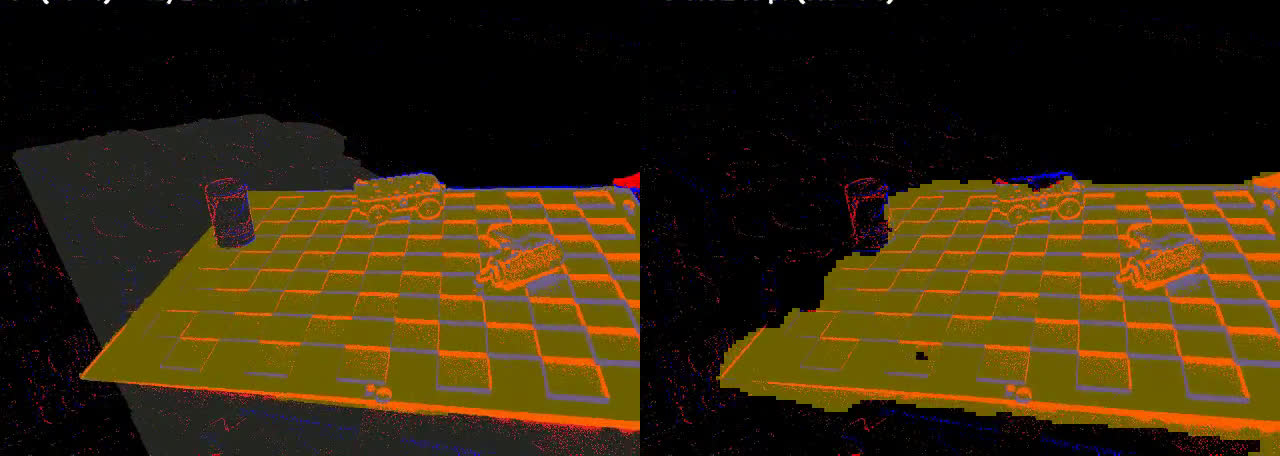
\includegraphics[width=0.49\textwidth]{figs/qual_1.jpg}}\hfill
\subfloat[]{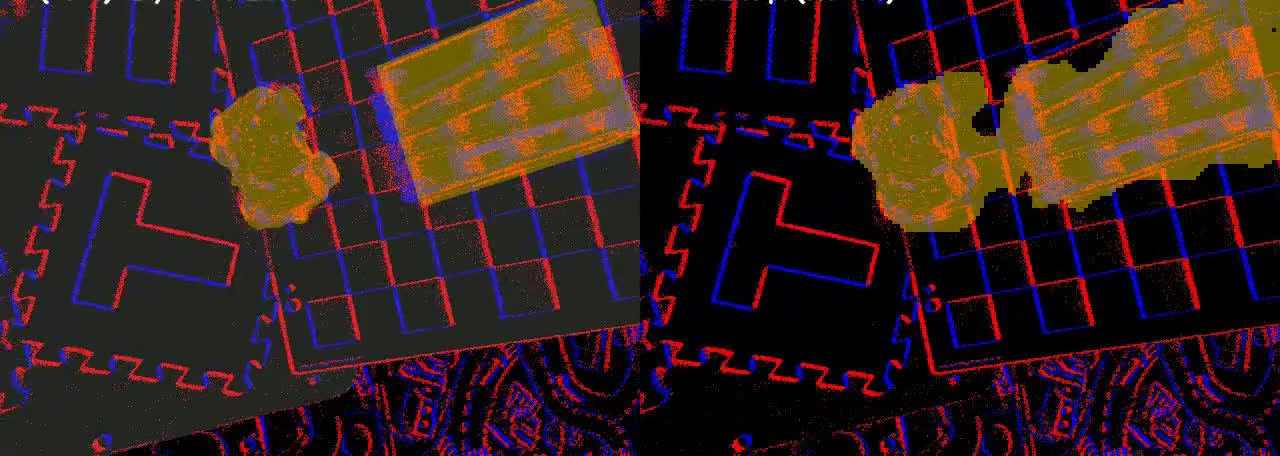
\includegraphics[width=0.49\textwidth]{figs/qual_2.jpg}}\\
\subfloat[]{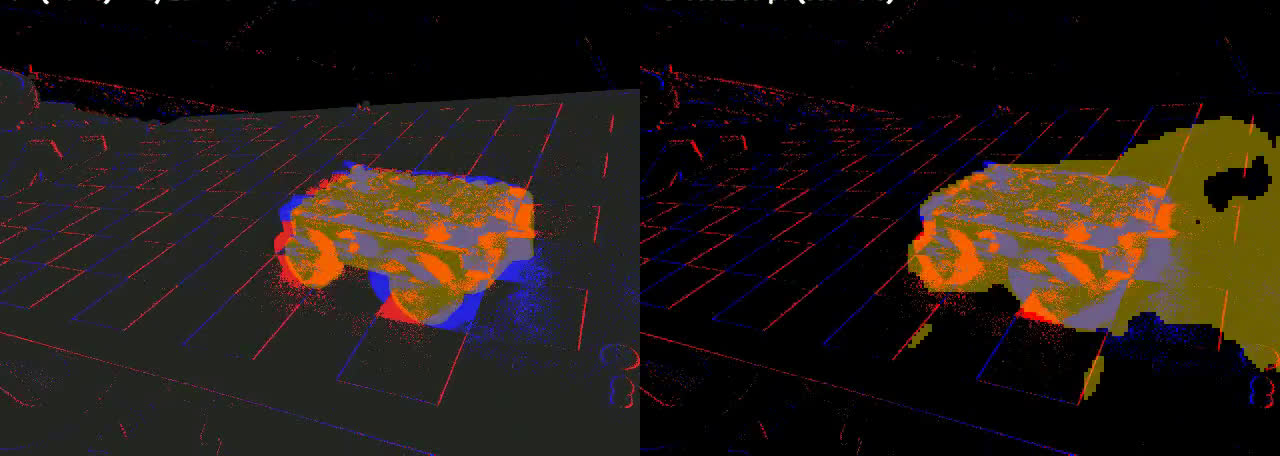
\includegraphics[width=0.49\textwidth]{figs/qual_3.jpg}}\hfill
\subfloat[]{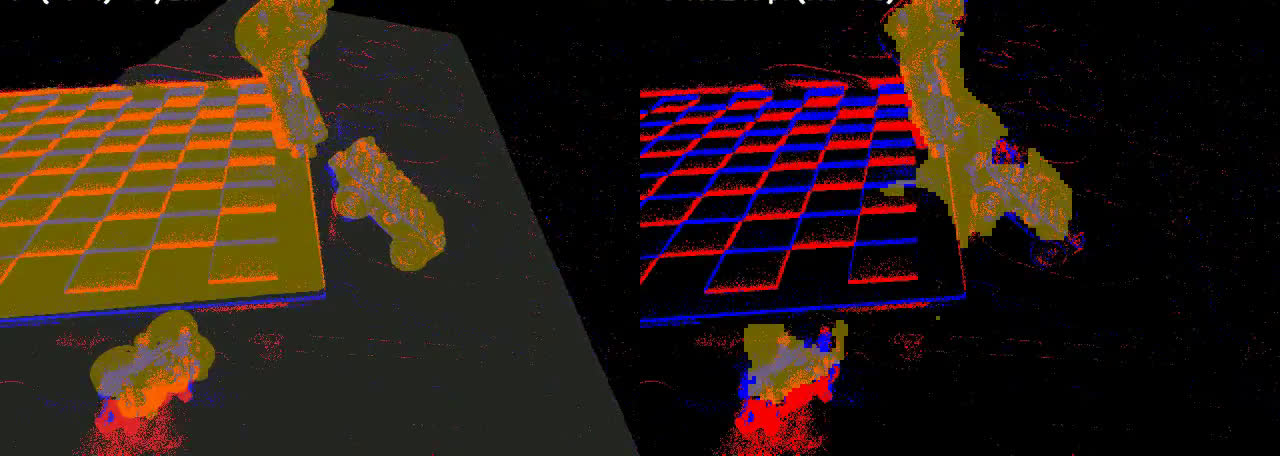
\includegraphics[width=0.49\textwidth]{figs/qual_4.jpg}}
\caption{Plug-in predictor M1 ($\wplus = 3$, seed 1) on EVIMO2 evaluation sequences.
Events in red and blue (polarity). Left of each pair: ground truth, with moving objects in
yellow and motion-captured objects that are static at this instant in gray (they would be
positive under the \code{all} definition). Right: cells where $p > 0.5$, in yellow; the
evaluation uses the continuous $p$. (a) a board moved as a whole is recovered; (b) two
objects moved together; (c) a moving car, with a false positive spilling over the static
background on its right; (d) failure: the small objects are detected but the large moving
board on the left is missed.}
\label{fig:qual}
\end{figure}

\begin{figure}[H]
\centering
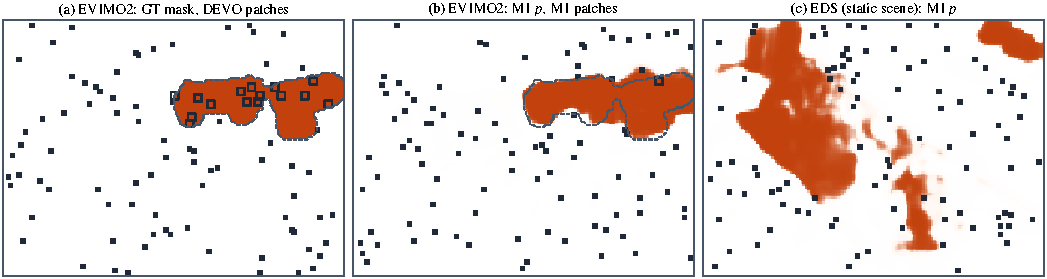
\includegraphics[width=\textwidth]{figs/scoremaps.pdf}
\caption{Patches selected by DEVO (squares) and dynamic probability (orange), one frame,
seed 1. (a) \code{scene14\_dyn\_test\_04}, ground-truth mask, pretrained DEVO: 15 of its 96
patches (hollow squares) lie on the moving objects. (b) Same frame, M1: $p$ covers the
objects (dashed: ground truth) and only one patch remains on them. (c) EDS
\code{11\_all\_characters}, a static scene: M1 flags 21\% of the cells of this frame as
moving, and the patches avoid the static structure under them. Over the 8 EVIMO2
sequences, 5.4\% of DEVO's patches fall on moving cells, 2.7\% with M1 and 0.7\% with the
oracle. Frame (a, b) chosen to illustrate the mechanism; frame (c) is the median frame of
its sequence.}
\label{fig:patches}
\end{figure}

\section{Cross-dataset results per sequence}

Tables below detail \cref{tab:cross} for the main methods. Each cell is the median over all
trials of all evaluation runs of that method (3 to 10 trials per run, 5 to 101 runs per
method and dataset). Best value of each row in bold. On TUM-VIE, the sequences
\code{mocap-shake}, \code{mocap-shake2}, \code{office-maze}, \code{running-easy},
\code{running-hard}, \code{skate-easy} and \code{skate-hard} are excluded: every method,
pretrained DEVO included, ends above 60\,cm on them (ground truth with gaps, or DEVO losing
track).

\newcommand{\crosshead}{Sequence & DEVO & M1 ($\wplus$=3) & M1 ($\wplus$=7) & M1 \code{all} & DEVO-ft & M2 ($\wplus$=3) & M3 ($\wplus$=3) \\}

\begin{table}[H]
\centering
\caption{RPG stereo~\cite{zhou2018semidense}: ATE (cm) per sequence, median over all
trials of all runs.}
\begin{tabular}{lccccccc}
\toprule
\crosshead
\midrule
\code{bin} & \best{1.4} & \best{1.4} & 1.5 & \best{1.4} & 4.5 & 4.3 & 3.1 \\
\code{boxes1} & \best{0.9} & \best{0.9} & \best{0.9} & \best{0.9} & 2.1 & 2.2 & 2.1 \\
\code{boxes2} & \best{0.9} & 1.0 & \best{0.9} & \best{0.9} & 4.1 & 3.6 & 3.6 \\
\code{desk1} & \best{0.9} & \best{0.9} & \best{0.9} & \best{0.9} & 2.1 & 2.2 & 2.2 \\
\code{desk2} & \best{1.3} & \best{1.3} & \best{1.3} & 1.4 & 3.4 & 3.6 & 3.4 \\
\code{monitor1} & \best{0.5} & \best{0.5} & \best{0.5} & \best{0.5} & 1.1 & 1.2 & 1.1 \\
\code{monitor2} & \best{0.7} & \best{0.7} & \best{0.7} & \best{0.7} & 1.6 & 1.7 & 1.6 \\
\code{reader} & 1.3 & \best{1.2} & \best{1.2} & \best{1.2} & 3.0 & 3.0 & 3.1 \\
\bottomrule
\end{tabular}
\end{table}

\begin{table}[H]
\centering
\caption{MVSEC indoor flying~\cite{zhu2018mvsec}: ATE (cm) per sequence, median over all
trials of all runs.}
\begin{tabular}{lccccccc}
\toprule
\crosshead
\midrule
\code{indoor\_flying1} & \best{10.5} & 10.9 & 11.0 & 12.9 & 31.2 & 25.3 & 22.4 \\
\code{indoor\_flying2} & 16.6 & \best{14.0} & 15.7 & 18.5 & 41.3 & 32.3 & 36.3 \\
\code{indoor\_flying3} & \best{15.0} & 16.9 & 15.3 & 23.0 & 25.7 & 20.8 & 22.1 \\
\code{indoor\_flying4} & \best{12.7} & 13.2 & 13.8 & 13.5 & 98.2 & 95.3 & 92.5 \\
\bottomrule
\end{tabular}
\end{table}

\begin{table}[H]
\centering
\caption{EDS~\cite{hidalgo2022eds}: ATE (cm) per sequence, median over all trials of all
runs.}
\begin{tabular}{lccccccc}
\toprule
\crosshead
\midrule
\code{00\_peanuts\_dark} & \best{4.3} & 4.6 & 5.5 & 4.7 & 66.5 & 64.6 & 70.3 \\
\code{01\_peanuts\_light} & 23.6 & 22.8 & 23.7 & \best{22.3} & 150.1 & 135.1 & 150.5 \\
\code{02\_rocket\_earth\_light} & 76.3 & \best{70.6} & 96.4 & 108.5 & 112.4 & 107.3 & 114.1 \\
\code{03\_rocket\_earth\_dark} & \best{37.6} & 52.9 & 59.5 & 42.5 & 116.4 & 117.1 & 116.9 \\
\code{06\_ziggy\_and\_fuzz} & \best{11.3} & 11.8 & 11.8 & 12.9 & 174.2 & 150.3 & 170.9 \\
\code{07\_ziggy\_and\_fuzz\_hdr} & \best{26.0} & 27.7 & 33.6 & 39.2 & 141.9 & 141.7 & 141.9 \\
\code{08\_peanuts\_running} & \best{37.0} & 41.1 & 37.2 & 46.9 & 131.6 & 129.1 & 134.2 \\
\code{09\_ziggy\_flying\_pieces} & \best{10.6} & 11.0 & 12.1 & 15.0 & 122.9 & 117.7 & 124.4 \\
\code{11\_all\_characters} & 77.6 & \best{40.2} & 68.2 & 102.2 & 126.5 & 126.6 & 127.2 \\
\bottomrule
\end{tabular}
\end{table}

\begin{table}[H]
\centering
\caption{VECtor~\cite{gao2022vector}: ATE (cm) per sequence, median over all trials of all
runs.}
\begin{tabular}{lccccccc}
\toprule
\crosshead
\midrule
\code{corner\_slow} & \best{1.0} & 1.3 & 1.6 & 1.7 & 1.8 & 1.9 & 1.9 \\
\code{corridors\_dolly} & \best{55.6} & 69.1 & 84.6 & 110.7 & 978.1 & 826.9 & 911.3 \\
\code{corridors\_walk} & \best{192.6} & 230.6 & 216.9 & 195.3 & 947.6 & 944.3 & 931.8 \\
\code{desk\_fast} & \best{6.1} & 7.0 & 7.7 & 17.6 & 34.4 & 35.3 & 35.3 \\
\code{desk\_normal} & \best{1.0} & 1.1 & 1.3 & 1.9 & 2.5 & 2.3 & 2.4 \\
\code{hdr\_fast} & 7.2 & 6.4 & \best{6.1} & 8.5 & 21.6 & 19.4 & 21.5 \\
\code{hdr\_normal} & 5.1 & 4.6 & 5.9 & 6.5 & \best{1.8} & 2.1 & 2.1 \\
\code{mountain\_fast} & \best{17.1} & 17.5 & 17.6 & 22.9 & 38.5 & 37.4 & 37.8 \\
\code{mountain\_normal} & \best{0.8} & \best{0.8} & \best{0.8} & 1.5 & 1.4 & 1.3 & 1.5 \\
\code{robot\_fast} & \best{3.4} & 7.9 & 11.1 & 4.3 & 32.8 & 33.3 & 33.5 \\
\code{robot\_normal} & \best{2.4} & 5.7 & 4.6 & 5.5 & 7.9 & 12.9 & 15.4 \\
\code{school\_dolly} & \best{44.1} & 53.3 & 76.7 & 76.3 & 1066.2 & 1164.8 & 1236.6 \\
\code{school\_scooter} & 65.7 & 52.8 & \best{51.2} & 67.0 & 1133.7 & 958.4 & 1349.9 \\
\code{sofa\_fast} & \best{11.2} & 12.1 & 14.8 & 33.6 & 37.9 & 37.8 & 38.0 \\
\code{sofa\_normal} & \best{4.9} & 5.1 & 6.0 & 8.3 & 41.1 & 42.8 & 45.5 \\
\code{units\_dolly} & 209.8 & \best{181.4} & 203.5 & 199.2 & 1330.8 & 1309.0 & 1403.6 \\
\code{units\_scooter} & 308.9 & \best{203.3} & 207.3 & 220.7 & 1380.8 & 1244.9 & 1437.3 \\
\bottomrule
\end{tabular}
\end{table}

\begin{table}[H]
\centering
\caption{TUM-VIE, motion-capture sequences~\cite{klenk2021tumvie}: ATE (cm) per sequence,
median over all trials of all runs.}
\begin{tabular}{lccccccc}
\toprule
\crosshead
\midrule
\code{mocap-1d-trans} & \best{0.5} & \best{0.5} & \best{0.5} & \best{0.5} & 1.3 & 1.3 & 1.1 \\
\code{mocap-3d-trans} & \best{1.0} & 2.3 & 1.6 & \best{1.0} & 27.9 & 27.8 & 27.8 \\
\code{mocap-6dof} & \best{1.6} & \best{1.6} & \best{1.6} & \best{1.6} & 2.0 & 2.0 & 2.0 \\
\code{mocap-desk} & \best{1.8} & 1.9 & \best{1.8} & 1.9 & 14.9 & 14.6 & 13.7 \\
\code{mocap-desk2} & 1.1 & 1.1 & 1.1 & \best{1.0} & 11.6 & 11.2 & 10.9 \\
\bottomrule
\end{tabular}
\end{table}

\end{document}
